\documentclass{article}
\usepackage[top=3cm,bottom=3cm,left=3cm,right=3cm]{geometry}
\usepackage[utf8]{inputenc}
\usepackage[default]{sourcesanspro}
\usepackage[hidelinks]{hyperref}
\usepackage[acronym]{glossaries}
\usepackage{glossary-inline}
\usepackage{graphicx}
\usepackage{float}

\usepackage{biblatex}
\addbibresource{sources/references.bib}

\makeglossaries
\newacronym{3dcnn}{3D CNN}{3D Convolutional Neural Networks}
\newacronym{2dcnn}{2D CNN}{2D Convolutional Neural Networks}
\newacronym{lidar}{LIDAR}{Laser detection and ranging}

\setglossarystyle{inline}

\title{Point Cloud Labeling using 3D Convolutional Neural Network}
\author{Elie \textsc{Kadoche}, Thomas \textsc{Petiteau}}
\date{12/04/2020}

\begin{document}

\maketitle

\section{Introduction}
\label{sec:intro}

The segmentation and labelisation of point cloud is a challenging computational problem that could be one key problem in the future of Artificial Intelligence (AI). Being able to interpret an environment read through technologies like \gls{lidar} gives the ability to autonomous system to understand and navigate in their surroundings. The autonomous vehicles are a perfect example of such use and a lot of constructor bet on this type of technology.\\

Previous approach on the problem required previous knowledge on the point cloud such as normals, roundness, etc. In 2016, \citeauthor*{7900038} \cite{7900038} proposed a new approach of the problem using deep learning similar to the ones used on images. The novelty of their approach reside in the fact that no prior information on the point cloud is required. Their algorithm is split into three phases, it firsts computes the voxelization of the point cloud in order to obtain well defined grid. These grids are passed to a \gls{3dcnn} that classify them into the different categories studied.
Finally, the labels of each points is deduced from the output of the network.\\

In this article, we propose to test their approach and try it on more complex data. Our work can be found \href{https://github.com/XanX3601/point_cloud_labeling.git}{here}. The goal is to see if their approach holds on with more categories. The rest of this paper is organized as follow. In section~\ref{sec:summary} we summarize the approach \cite{7900038}. In section~\ref{sec:dataset} we describe our choosen dataset. In section~\ref{sec:implementation} we discuss our choices and problems in the implementation of the algorithm. In section~\ref{sec:results} we reveal the results of our experiments on a new dataset of point cloud. In section~\ref{sec:future} we expose some ideas for future work that may lead to an improvement of the global performance. In section~\ref{sec:conclusion} we conclude this article.

\section{Labeling point cloud with \gls{3dcnn}}
\label{sec:summary}

The approach presented by \citeauthor*{7900038} is composed of two steps which is very classic when working with neural networks. The first step aims to train the neural network on training data that need to be computed beforehand. The second is the exploitation of the trained network to label new point clouds.

\subsection{Point cloud preprocessing and voxelization}

In order to use a convolution operation, we need a well defined matrix filled with values. A point cloud is not a well defined grid, its shape is irregular and therefore, a convolution operation is hard to compute directly on the raw data. A first approach was to project the three dimensional data into depth images which are well defined grids of pixels that can be treated by two dimensional convolution. Projecting data on smaller space mean that there is a lost of information. The challenge is to extract structures that can easily be used into three dimensional convolution from a point cloud.\\

The voxelization of a point cloud brings a regular grid around a point cloud where each cell, called voxel, represents a single value. As it is a regular grid, it can be passed through a convolution operation. Therefore, the step needed before using a \gls{3dcnn} on the data is to compute a voxel grid that can be seen as a matrix. The size and shape of a point cloud being seriously inconsistent, the entire voxel grid cannot be processed at once. A \gls{3dcnn} is much easier to use when the inputs are consistent in size. The ingenious idea depicted \cite{7900038} is to compute a voxel grid on the entire cloud point, attribute a value and a label to each cell and then extract sub-grid that can be fed to the network.\\

To compute the entire voxel grids, a box bound containing the entire point cloud must be computed and it is then used to place the centers of each voxel on the grid. The entire bound box is densely sampled by voxel of size \(\frac{R}{N} * \frac{1}{2}\). To attribute values to each voxel, \citeauthor*{7900038} explain two approaches. First, one can put 1 in a voxel containing at least a point and 0 otherwise. Secondly, one can count the number of points in a voxel and set its value to its density.\\

Having a value set for each voxel, the next step is to attribute a label to each one. The simplest way to do so is to count the number of occurrences of each label inside a voxel and elect the most frequent one. If an equality occur, a random one can be attributed among the most frequent.\\

The last step is to extract sub-grids that can be fed to network later on. To do so, for each voxel of center \((x, y, z)\), we consider a box defined by \([x - \frac{R}{2}, x + \frac{R}{2}] \times [y - \frac{R}{2}, y + \frac{R}{2}] \times [z - \frac{R}{2}, z + \frac{R}{2}]\) which is composed of \(N \times N \times N\) voxels. Theses sub-grids can be extracted for each voxel and are labeled as the voxel in their centre.

\subsection{The \gls{3dcnn}}

Once that all the voxel grids are extracted from the point cloud, they can be passed to the network. The one used by \citeauthor*{7900038} is fairly simple and is composed of two 3D convolutional layers, two 3D pooling layers and one fully-connected layer. It looks strongly alike to any \gls{2dcnn} used on images. This network takes matrices of size \((1 \times N \times N \times N)\) and outputs a probability distribution over the different labels.

\subsection{Infer label using the network}

We can finally use the neural network to labelize a new point cloud. We follow the same voxelization step we have just described. After that, the process is pretty straightforward, we simply label each point in the voxel at the center of each grid with the label given by the network.

\section{The Virtual KITTI 3D Dataset}
\label{sec:dataset}

For their experiments, the authors decided to use the large \gls{lidar} point cloud dataset of the urban area of Ottawa. This large dataset allowed the authors to balanced the samples used for training: the idea is to have the same amount of samples for each label. We needed to find a dataset large enough and interesting enough to be adequate.\\

We finally decided to use the Virtual KITTI 3D Dataset for Semantic Segmentation. More information about it can be found \href{https://github.com/VisualComputingInstitute/vkitti3D-dataset.git}{here}. This dataset contains labelled point clouds of vehicles surroundings. We decided to use this dataset for 4 main reasons.
\begin{itemize}
    \item[\(\bullet \)] It is simple to use, we created scripts to exploit and visualize it easily.
    \item[\(\bullet \)] It is an interesting dataset since it can directly be related to the actual autonomous vehicle challenge.
    \item[\(\bullet \)] It is a more complex dataset since there are 13 possible classes (compare to 7 for the one useb by the authors) and it is then more complicated to balance the samples.
    \item[\(\bullet \)] It looks nice, as you can see in the figures \ref{pic1} and \ref{pic2}.
\end{itemize}

\begin{figure}[H]
    \centering
	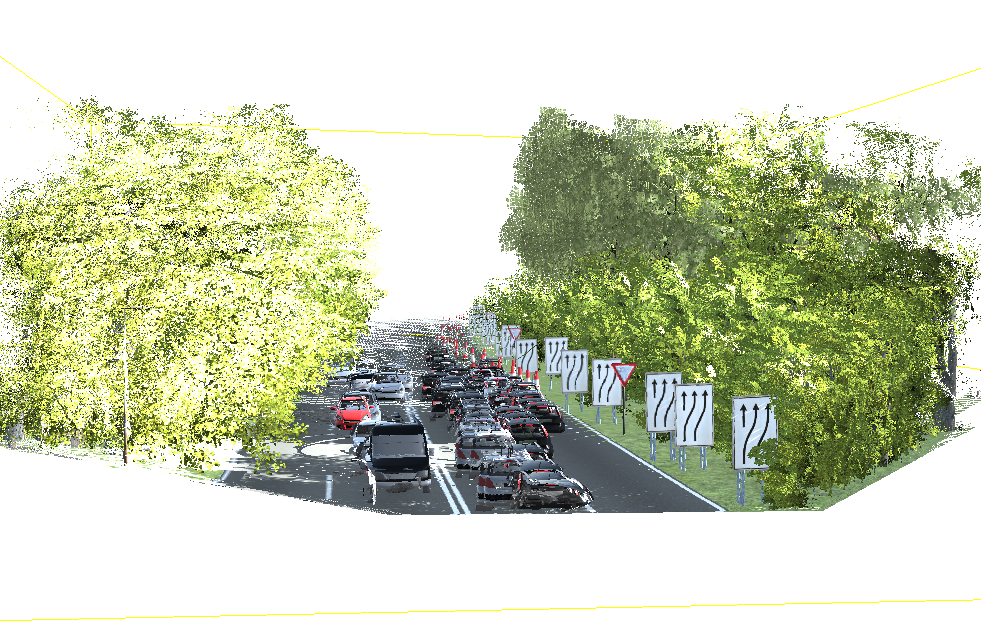
\includegraphics[scale=0.3]{sources/pic1.png}
	\caption{Point cloud colorized}
	\label{pic1}
\end{figure}

\begin{figure}[H]
    \centering
	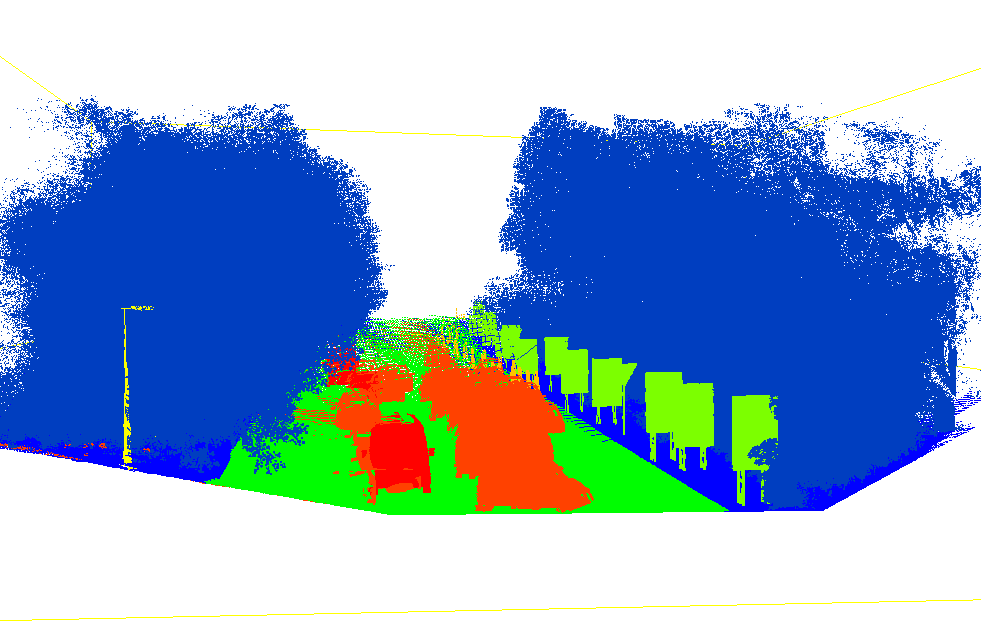
\includegraphics[scale=0.3]{sources/pic2.png}
	\caption{Point cloud labelized}
	\label{pic2}
\end{figure}

\section{Implementation choices}
\label{sec:implementation}

In this section we discuss the choices we made for implementing the algorithm \cite{7900038}.
We will also discuss the problems we encounter in the comprehension of the article or while programming.

\subsection{Training datasets}

In their article, \citeauthor*{7900038} suggest to balance the number of training samples between each category. This is to ensure that the network is trained evenly on all classes and that it does not learn any bias towards the most frequent classes. We agree on this point and tried to implement this balance. The problem is that, in our dataset, the class frequencies are highly uneven.
Moreover, when creating training samples from cloud point, we obtain a lot of samples from different classes. With our computation power, we could not afford to save all the samples in one place. We were then in the incapacity to sort training samples after-hand, once they were all extracted. We decided to choose the training samples randomly with a bias towards the class appearing less often. Our goal is to elect an even number of voxel for each class. To do so, we suppose that the distribution of classes over the point will be mostly the same with voxels. We then elect a voxel to be a training sample by choosing a random number between 0 and 1 that needs to be lower than \(\frac{n_{j}}{\min_{i \in L}(n_{i})}\) where \(n_{i}\) is the number of points with label \(i\), \(L\) is the set of labels and \(j\) is the label of the voxel. Unfortunately, this solution, although it let us pick a reasonable amount of training samples, it does not ensure the balanced between categories. The problem being that, for certain category, the amount of available voxels will be limited and thus, we cannot ensure a good balance between number of training samples and the even amount of training samples per class.

\subsection{Story of granularity}

In their article, \citeauthor*{7900038} speak, in section VI, dedicated to the label inference, of an alternative to the compact division of the point cloud. In the voxelization process, the point cloud is divided into a lot of voxels. The number increases rapidly and can quickly become a problem for low specs machine. Therefore, an approach that would give close results in less time, would be interesting. The granularity seems to be a solution they found but they don't give a proper explanation in their experiments.

\subsection{KDTree for cubes}

In order to compute the voxelization, an easy way to find to which voxel a point belong is to use a KDTree. Combine with a Chebyshev distance, it allows to quickly find all the points in a cube.
At first, we did not use a KDTree and it multiplied the computation time needed for voxelization by an enormous factor.

\section{Experiments and results}
\label{sec:results}

The Virtual KITTI 3D Dataset is split into 6 different point clouds. For our experiments, we used 5 for training the neural network and 1 for testing it. Below there are some of our results. In pictures \ref{res_true} and \ref{res1_pred}, we can see the result is not visually pleasing but overall, the algorithm seems to distinguish easily the trees from the rest. We can also see that a pole in the left side is quite recognizable. However, in picture \ref{res2_pred}, we begin to see better classification. It gives us good hope on the algorithm, since picture \ref{res2_pred} was computed on more samples (but more unbalanced). Then, we might think that with more balanced data, we could achieve expected results.\\

We explain the quality of our results by the strong imbalance of our dataset. We logged information about our training dataset in \verb|.info| files and we saw that the tree classs is the most predominant one. It is then difficult to have training samples balanced over all the labels. The authors took 50000 balanced training samples, and we have barely 20000 samples, which are not even well balanced. Another issue is the required computing power: we lack a beautiful RTX 2080 Ti and some RAM. But we managed to use Google Colab to train some models and obtain some results.

\begin{figure}[H]
    \centering
	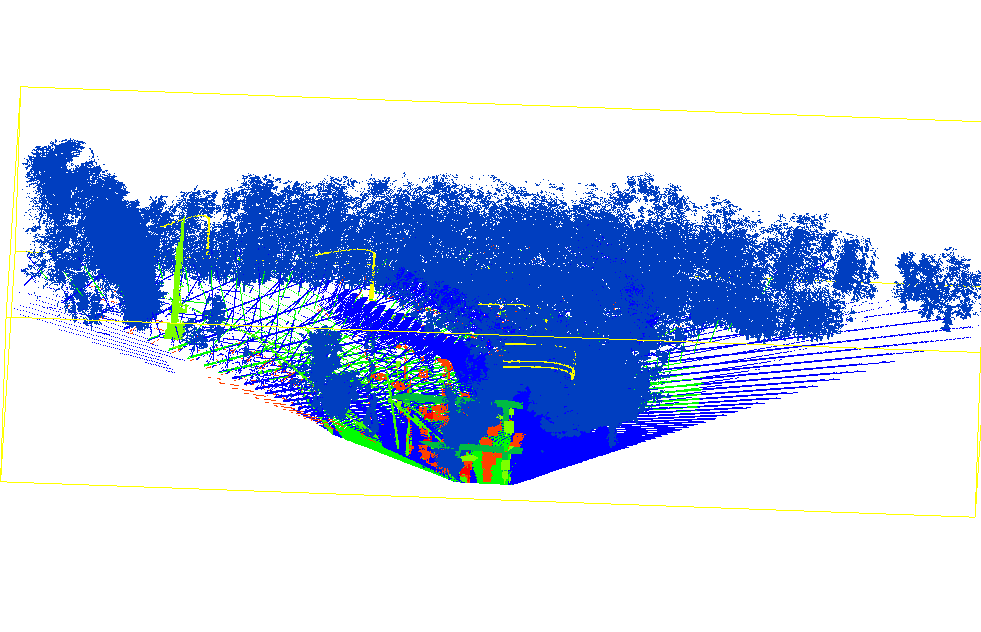
\includegraphics[scale=0.27]{sources/res_true.png}
	\caption{Experiment 1: true labels}
	\label{res_true}
\end{figure}

\begin{figure}[H]
    \centering
	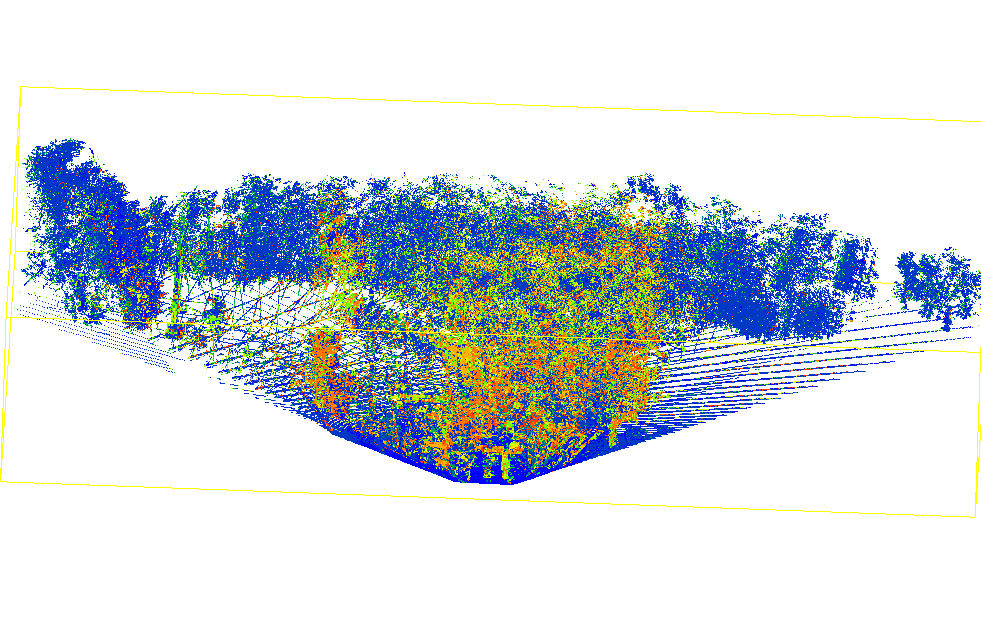
\includegraphics[scale=0.27]{sources/res1_pred.png}
	\caption{Experiment 1: predicted labels}
	\label{res1_pred}
\end{figure}

\begin{figure}[H]
    \centering
	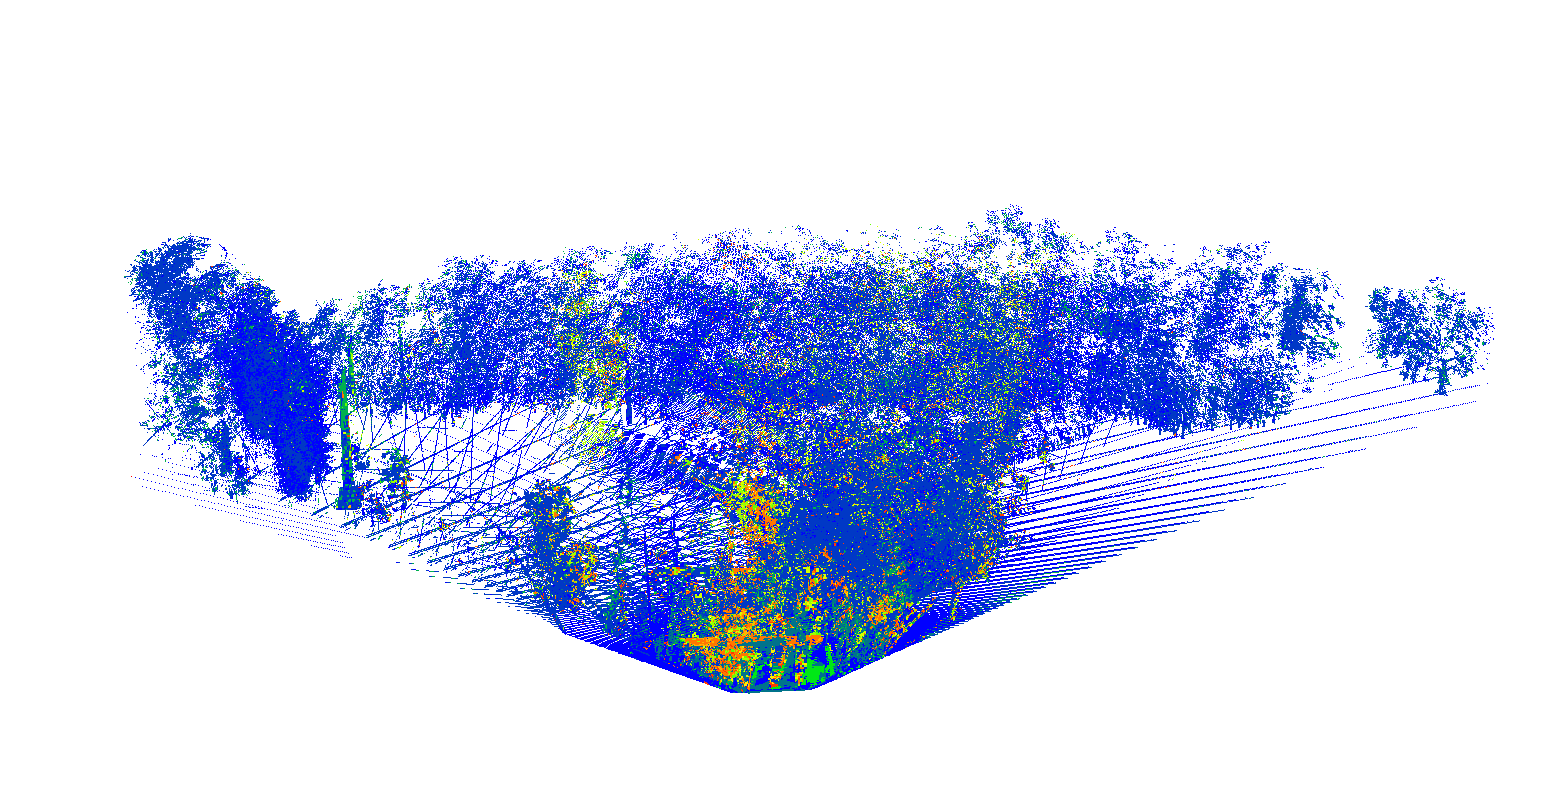
\includegraphics[scale=0.27]{sources/res2_pred.png}
	\caption{Experiment 1: predicted labels}
	\label{res2_pred}
\end{figure}

\section{Future work}
\label{sec:future}

In the future, there are different ideas we would like to try in order to improve the performance of the approach. Changing the way of setting the voxel value during the voxelization step could put more information into the matrix. As suggested, changing the values to the density of points in each voxel would help to differentiate dense structure from clearer ones. We would like to study the augmentation of channels on the voxel. We think that including information such as colors, which is very common in images study, could lead to a big boost of performance. A simple operation as setting the value of each voxel to the average color of the points it contains may be sufficient to observe better performances.

\section{Conclusion}
\label{sec:conclusion}

In this article, we tested an approach suggested by \citeauthor*{7900038} in an article \cite{7900038} in 2016. They used a \gls{3dcnn} to labelize each point of a cloud. Their algorithm does not require prior knowledge on the cloud which is new in the approach of the problem. Previously, a certain numbers of features would be required and thus, would require computation time. With this new strategy, they reduce the computation time to a few minutes. Their approach consists in voxelizing the point cloud and feed cube of voxels to a neural network that use convolution in way that is similar to what neural networks already do on 2D images. The prediction of the network are then used to set the label of the points at the center of the cube used in input.\\

We implemented their algorithm and we tested it on a dataset with twice more categories, and a strong ubalanced labels repartition. We found this approach very interested, and we think we managed to implement it in a efficient way. Unfortunately, we did not manage to get the expected results. We explain this by the dataset properties and the lack of computation power.\\

PointNet \cite{qi2016pointnet}, proposes a another kind of neural network fixing some of the issues of the presented method. PointNet allows to consume point clouds directly, without having to transform it in a regular 3D voxel grids. Such a method might be a better approach, simpler and more efficient.


\printglossaries
\printbibliography

\end{document}
